
	\documentclass{article}

	\usepackage{multicol}
    \usepackage{color}
    \usepackage{graphics}

    \definecolor{dkgreen}{rgb}{0,0.6,0}
    \definecolor{gray}{rgb}{0.5,0.5,0.5}
    \definecolor{mauve}{rgb}{0.58,0,0.82}
    
	\usepackage[paperheight=27.94cm,paperwidth=21.59cm,left=3.0cm,right=3.0cm,top=2.5cm,bottom=2.5cm]{geometry}
	
	\setlength\parindent{0pt}
	\renewcommand{\arraystretch}{1.3}
	
	\usepackage{listings}
	
\begin{document}



\title{Distributed and Partitioned Key-Value Store \\ \large{Parallel and Distributed Computing}
\\ \large{2nd Project Report}}



\author{Henrique Sousa, Mateus Silva, Melissa Silva}
\date{Porto, June 3rd 2022}
\date{\textbf{Teacher} Jorge Barbosa}

\maketitle

\begin{multicols}{2}

	\section{Membership Service}

	Since the goal of the project is the development of a distributed and persistent key-value store for a large cluster, it’s required that every node knows every other node inside the cluster. To accomplish this, the nodes run a distributed membership service and protocol. \\

	The Membership Service supports two distinct operations:
	\textit{join()}, which adds a node to the cluster, and \textit{leave()}, which removes a node from the cluster. \\
	
	Every time a node chooses to join or leave the cluster, a specific message detailing which operations it would like to do must be sent.

	\subsection{Message Structure}
	
	\subsubsection{Join \& Leave}
	Each message has four arguments:

	\begin{itemize}
		\item The operation declaration (either \textit{join} or \textit{leave});
		\item An identifier of the node who will perform the operation;
		\item The membership counter;
		\item The local port of the TCP socket.
	\end{itemize}
	
	The membership counter value helps determine which operation occurred – an even value means the node just \textbf{joined} the cluster and that it \textbf{left} the cluster otherwise.

	\subsubsection{Membership}
	These messages are sent in response to the \textit{join} message the cluster nodes receive by an outside node, so their structure is different from the one used for \textit{join} and \textit{leave} and one of the several types of messages made using the \textit{Message} class, each type having both a header and a body.\\
	
	The header only includes the message’s subject, \textit{MEMBERSHIP}. The body includes information from the \textit{MembershipData} class: the 32 most recent membership events in the membership logs and a list of the current members in the cluster. This information is translated into a string which is then sent.

	\subsection{Membership Log}
	Upon receiving a \textit{join} or \textit{leave} message, the cluster node adds an entry in the membership log specifying the last action.\\
	
	Each entry includes the operation value (\textit{join} or \textit{leave}), the node’s \textit{id} and the value of the membership counter.

	\lstinputlisting[frame=tb,
    language=Java,
    aboveskip=3mm,
    belowskip=3mm,
    showstringspaces=false,
    columns=flexible,
    basicstyle={\small\ttfamily},
    numbers=none,
    numberstyle=\tiny\color{gray},
    keywordstyle=\color{blue},
    commentstyle=\color{dkgreen},
    stringstyle=\color{mauve},
    breaklines=true,
    breakatwhitespace=true,
    tabsize=3,
    linerange={1-4}
    ]{input.java}
    \textbf{Note:}{ Code edited to fit formatting (explicit class invocation).}

	\subsection{Message Handling}
	The transfer of membership information is done using TCP. \\
	
	A new member sends the request to \textit{join} message using this protocol and the cluster members send information back in the same way. These don’t, however, send it right away, opting instead to wait a \textbf{random} time length before doing so.\\
	
	A connection between a new node and the cluster members is broken after reception of 3 \textit{MEMBERSHIP} messages.\\
	
	In case this trio of information never arrives, the new node repeats transmission of the \textit{join} message for, at max, two more times, making it a total of \textbf{three attempts} at getting a response from the cluster.
	
	\subsection{Stale Membership Information}
	Outdated nodes will not provide confirmation to a joining node.\\
	
	A node calculates if they are outdated or not --- this happens when a node hasn't received a membership update for 1.5 times the periodicity of the membership update \textit{multicast} messages.

    \subsection{Initialization + Extra Feature}
    The very first node joining the cluster will not be able to receive any membership message. Thus, for any node that does not receive the required number of confirmations to join the cluster, initialization is made as if it is the only node in the cluster. \\
    
    Beyond being a neat solution for the cluster creator, it also addresses problems when a node was not able to receive the required confirmations: the node will still join the cluster and, as membership updates arrive, the node will eventually reach the current state of the cluster. \\
    
    Additionally, to create a more controlled environment, we provide another operation to the test client: a \textit{create} operation that allows instant creation of the cluster without any confirmation hindrances. \\
    \subsection{Fault Tolerance}
    \subsubsection{Clusters Under 3 Members}
    When a node joins a cluster with less than 3 members, there will not be 3 confirmations: \textit{MembershipData} is analyzed for each of the confirmations received. \\
    
    If the number of nodes indicated by the confirmations is under 3, then the joining node will adjust the needed number of confirmations. \\
    
    Even though with just 3 required confirmations this problem is reduced, for larger amounts, this solution provides an adaptable way to have a seamless joining procedure.
    
    \subsubsection {Membership Updates}
    To ensure that all the nodes are away of the updated cluster status, we adopted a \textit{brute-force} approach. \\
    
    What we mean by this is that every node will periodically share their status to the whole network. Due to the incremental nature of the logs, the status is a monotonic function that will only vary towards the most up to date state. \\
    
    Missing some of the membership update messages is not critical since the node will be able to use other nodes to update its status.

	\section{Storage Service}
	A normal execution will have the following steps:
	\begin{enumerate}
	    \item In case of a \textit{put}:
	    \begin{enumerate}
	        \item \textit{Client} sends a PUT message to a node with the name of the file and the file path;
	        \item \textit{Node} hashes the filename, obtains the node the operation must be sent to and sends a CLUSTER\_PUT to that node.
	        \item The other node receives the request and processes it, storing the file in memory and obtaining the storage key. It then does two things:
	        \begin{enumerate}
	            \item First, it replies to the first node with a PUT\_RESPONSE;
	            \item Next, it informs its neighbors of the operation with a PUT\_INFORM;
	        \end{enumerate}
	        \item Finally, the first node that was contacted receives the PUT\_RESPONSE. From the request number, it is able to identify the socket of the client where the request came from and send the hash back to them.
	    \end{enumerate}
	\end{enumerate}
	The process for other operations is analogous. \textbf{Page 5} includes the message structure used for all operations.
	
	\subsection{Fault Tolerance}
	\subsubsection{\textit{Get} Operation to Crashed Node}
    It might happen that a \textit{get} request cannot be fulfilled. \\
    
    This can happen for two reasons:
    \begin{enumerate}
        \item The node has crashed before the node requesting a file has had time to register the change;
        \item The node was able to establish a TCP connection, but the node crashed in the meantime.
    \end{enumerate}
    To guarantee that requests under these situations are fulfilled, we implemented a timeout in the request: if there is a timeout, the node will ask the neighbors of the crashed node for the needed information. Since keys are replicated, they will be able to provide it.

    \section{Replication}
    Replication is possible in only two circumstances: when a key-value pair is updated, or when a node leaves or joins the cluster.\\
    
    Considering the existence of replication and multiple ownership of a key-value, we defined the original owner as the node whose hash is closest to the one of the key-value - this is the node described in \textbf{Chapter 4} of the project description.

    \subsection{Key-Value Update}
    Key-value pairs are updated whenever a \textit{put} or \textit{delete} operation happens; however, there might be a difference whenever a node receives either operation. \\
    
    The node that receives the operation might be the original owner, in which case it will update its neighbors. \\ 
    
    Otherwise, the node receiving the operation is one of the neighbors receiving the update.
    \lstinputlisting[frame=tb,
    language=Java,
    aboveskip=3mm,
    belowskip=3mm,
    showstringspaces=false,
    columns=flexible,
    basicstyle={\small\ttfamily},
    numbers=none,
    numberstyle=\tiny\color{gray},
    keywordstyle=\color{blue},
    commentstyle=\color{dkgreen},
    stringstyle=\color{mauve},
    breaklines=true,
    breakatwhitespace=true,
    tabsize=3,
    linerange={7-19}
    ]{input.java}
    \textbf{Note:}{ == was used instead of \textit{.equals()} for formatting purposes.} 
    
    \section{Membership Updates}
    Any change within the cluster causes replication of keys. In case of a \textit{join}, each node who is already in the cluster evaluates if the joining node is its neighbor. \\
    
    In that case, it will replicate its original keys \footnote{As in keys originally owned by the node.} to the newly joined node.  \\
    
    There will be no attempt at removing replicas that are now outdated.
    \lstinputlisting[frame=tb,
    language=Java,
    aboveskip=3mm,
    belowskip=3mm,
    showstringspaces=false,
    columns=flexible,
    basicstyle={\small\ttfamily},
    numbers=none,
    numberstyle=\tiny\color{gray},
    keywordstyle=\color{blue},
    commentstyle=\color{dkgreen},
    stringstyle=\color{mauve},
    breaklines=true,
    breakatwhitespace=true,
    tabsize=3,
    linerange={21-28}
    ]{input.java}
    \textbf{Note:}{ == was used instead of \textit{.equals()} for formatting purposes.} \\
    
    In case of a \textit{leave}, each node in the cluster will evaluate if the leaving node is its neighbor. In that case, then it will replicate its original keys to the \textbf{second neighbor} of the leaving node, hence \textit{“replacing”} (in practice) the leaving node.
    \lstinputlisting[frame=tb,
    language=Java,
    aboveskip=3mm,
    belowskip=3mm,
    showstringspaces=false,
    columns=flexible,
    basicstyle={\small\ttfamily},
    numbers=none,
    numberstyle=\tiny\color{gray},
    keywordstyle=\color{blue},
    commentstyle=\color{dkgreen},
    stringstyle=\color{mauve},
    breaklines=true,
    breakatwhitespace=true,
    tabsize=3,
    linerange={30-40}
    ]{input.java} \\
    
    Additionally, the leaving node will also replicate its original keys to \textbf{three nodes}: their new original owner and its two neighbors. 
    
    \lstinputlisting[frame=tb,
    language=Java,
    aboveskip=3mm,
    belowskip=3mm,
    showstringspaces=false,
    columns=fullflexible,
    basicstyle={\small\ttfamily},
    numbers=none,
    numberstyle=\tiny\color{gray},
    keywordstyle=\color{blue},
    commentstyle=\color{dkgreen},
    stringstyle=\color{mauve},
    breaklines=true,
    breakatwhitespace=true,
    tabsize=3,
    linerange={42-53}
    ]{input.java}
    \textbf{Note:}{ Line breaks added for formatting purposes.}
    
    \section{Concurrency}
    
    \subsection{\textit{Thread Pools}}
    Overall, we have a single \textit{thread pool} to which tasks are added accordingly. At the time of writing, it uses six total threads. \\
    
    There is a thread assigned to each of the two open sockets (one UDP and one TCP) to handle the reception of messages. The threads will constantly listen on the respective socket, waiting for a packet or message. Upon receiving either one, it will dedicate a new thread on the pool to process the received information.\\
    
    We chose this approach since it resembles having a single dispatcher where handling of any outside connection does not warrant delays, since the thread is always listening for new information: for example, when the TCP socket is open, we'll prepare to receive information on it first.

    \lstinputlisting[frame=tb,
    language=Java,
    aboveskip=3mm,
    belowskip=3mm,
    showstringspaces=false,
    columns=flexible,
    basicstyle={\small\ttfamily},
    numbers=none,
    numberstyle=\tiny\color{gray},
    keywordstyle=\color{blue},
    commentstyle=\color{dkgreen},
    stringstyle=\color{mauve},
    breaklines=true,
    breakatwhitespace=true,
    tabsize=3,
    linerange={55-71}
    ]{input.java}
    \textbf{Note:}{ Line breaks added for formatting purposes.}
    \break
    Then, the reader will be permanently trying to assemble a valid message, the structure of which has been described previously. 
    \lstinputlisting[frame=tb,
    language=Java,
    aboveskip=3mm,
    belowskip=3mm,
    showstringspaces=false,
    columns=flexible,
    basicstyle={\small\ttfamily},
    numbers=none,
    back
    numberstyle=\tiny\color{gray},
    keywordstyle=\color{blue},
    commentstyle=\color{dkgreen},
    stringstyle=\color{mauve},
    breaklines=true,
    breakatwhitespace=true,
    tabsize=3,
    linerange={73-75}
    ]{input.java}
    If it succeeds, the handling of the message will be handed to the \textit{membershipProtocol} which will create another thread. 
    \lstinputlisting[frame=tb,
    language=Java,
    aboveskip=3mm,
    belowskip=3mm,
    showstringspaces=false,
    columns=flexible,
    basicstyle={\small\ttfamily},
    numbers=none,
    numberstyle=\tiny\color{gray},
    keywordstyle=\color{blue},
    commentstyle=\color{dkgreen},
    stringstyle=\color{mauve},
    breaklines=true,
    breakatwhitespace=true,
    tabsize=3,
    linerange={77-79}
    ]{input.java}
    The process is the same for the three threads handling the reception of information through a socket.
    
    \section{Fault Tolerance}
    \subsection{Message Sent to Wrong Destination}
    Every operation sent through TCP features the node that the message was (originally) sent to. If the receiving node notices that they aren't the indicated destination, the message will be redirected to the right one.
    
	\section{Conclusion}
	This was a very challenging project, especially in all the testing made for it - we invested some time into figuring out the best way to test our code and automate this process for efficiency purposes. \\
	
    We did have a chance to apply concepts learned in theory classes, specifically, the class lectured by Prof. Fahed Jubair.
    \end{multicols}
    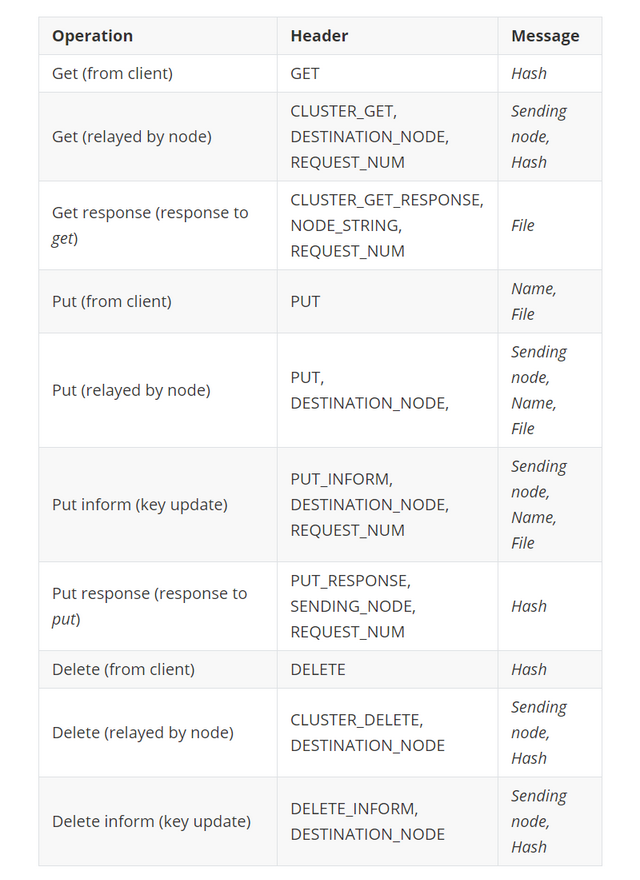
\includegraphics{tabela.png}
\end{document}

